% Options for packages loaded elsewhere
\PassOptionsToPackage{unicode}{hyperref}
\PassOptionsToPackage{hyphens}{url}
\PassOptionsToPackage{dvipsnames,svgnames,x11names}{xcolor}
%
\documentclass[
  a4paper,
  DIV=11,
  numbers=noendperiod]{scrartcl}

\usepackage{amsmath,amssymb}
\usepackage{iftex}
\ifPDFTeX
  \usepackage[T1]{fontenc}
  \usepackage[utf8]{inputenc}
  \usepackage{textcomp} % provide euro and other symbols
\else % if luatex or xetex
  \usepackage{unicode-math}
  \defaultfontfeatures{Scale=MatchLowercase}
  \defaultfontfeatures[\rmfamily]{Ligatures=TeX,Scale=1}
\fi
\usepackage{lmodern}
\ifPDFTeX\else  
    % xetex/luatex font selection
\fi
% Use upquote if available, for straight quotes in verbatim environments
\IfFileExists{upquote.sty}{\usepackage{upquote}}{}
\IfFileExists{microtype.sty}{% use microtype if available
  \usepackage[]{microtype}
  \UseMicrotypeSet[protrusion]{basicmath} % disable protrusion for tt fonts
}{}
\makeatletter
\@ifundefined{KOMAClassName}{% if non-KOMA class
  \IfFileExists{parskip.sty}{%
    \usepackage{parskip}
  }{% else
    \setlength{\parindent}{0pt}
    \setlength{\parskip}{6pt plus 2pt minus 1pt}}
}{% if KOMA class
  \KOMAoptions{parskip=half}}
\makeatother
\usepackage{xcolor}
\setlength{\emergencystretch}{3em} % prevent overfull lines
\setcounter{secnumdepth}{-\maxdimen} % remove section numbering
% Make \paragraph and \subparagraph free-standing
\ifx\paragraph\undefined\else
  \let\oldparagraph\paragraph
  \renewcommand{\paragraph}[1]{\oldparagraph{#1}\mbox{}}
\fi
\ifx\subparagraph\undefined\else
  \let\oldsubparagraph\subparagraph
  \renewcommand{\subparagraph}[1]{\oldsubparagraph{#1}\mbox{}}
\fi

\usepackage{color}
\usepackage{fancyvrb}
\newcommand{\VerbBar}{|}
\newcommand{\VERB}{\Verb[commandchars=\\\{\}]}
\DefineVerbatimEnvironment{Highlighting}{Verbatim}{commandchars=\\\{\}}
% Add ',fontsize=\small' for more characters per line
\usepackage{framed}
\definecolor{shadecolor}{RGB}{241,243,245}
\newenvironment{Shaded}{\begin{snugshade}}{\end{snugshade}}
\newcommand{\AlertTok}[1]{\textcolor[rgb]{0.68,0.00,0.00}{#1}}
\newcommand{\AnnotationTok}[1]{\textcolor[rgb]{0.37,0.37,0.37}{#1}}
\newcommand{\AttributeTok}[1]{\textcolor[rgb]{0.40,0.45,0.13}{#1}}
\newcommand{\BaseNTok}[1]{\textcolor[rgb]{0.68,0.00,0.00}{#1}}
\newcommand{\BuiltInTok}[1]{\textcolor[rgb]{0.00,0.23,0.31}{#1}}
\newcommand{\CharTok}[1]{\textcolor[rgb]{0.13,0.47,0.30}{#1}}
\newcommand{\CommentTok}[1]{\textcolor[rgb]{0.37,0.37,0.37}{#1}}
\newcommand{\CommentVarTok}[1]{\textcolor[rgb]{0.37,0.37,0.37}{\textit{#1}}}
\newcommand{\ConstantTok}[1]{\textcolor[rgb]{0.56,0.35,0.01}{#1}}
\newcommand{\ControlFlowTok}[1]{\textcolor[rgb]{0.00,0.23,0.31}{#1}}
\newcommand{\DataTypeTok}[1]{\textcolor[rgb]{0.68,0.00,0.00}{#1}}
\newcommand{\DecValTok}[1]{\textcolor[rgb]{0.68,0.00,0.00}{#1}}
\newcommand{\DocumentationTok}[1]{\textcolor[rgb]{0.37,0.37,0.37}{\textit{#1}}}
\newcommand{\ErrorTok}[1]{\textcolor[rgb]{0.68,0.00,0.00}{#1}}
\newcommand{\ExtensionTok}[1]{\textcolor[rgb]{0.00,0.23,0.31}{#1}}
\newcommand{\FloatTok}[1]{\textcolor[rgb]{0.68,0.00,0.00}{#1}}
\newcommand{\FunctionTok}[1]{\textcolor[rgb]{0.28,0.35,0.67}{#1}}
\newcommand{\ImportTok}[1]{\textcolor[rgb]{0.00,0.46,0.62}{#1}}
\newcommand{\InformationTok}[1]{\textcolor[rgb]{0.37,0.37,0.37}{#1}}
\newcommand{\KeywordTok}[1]{\textcolor[rgb]{0.00,0.23,0.31}{#1}}
\newcommand{\NormalTok}[1]{\textcolor[rgb]{0.00,0.23,0.31}{#1}}
\newcommand{\OperatorTok}[1]{\textcolor[rgb]{0.37,0.37,0.37}{#1}}
\newcommand{\OtherTok}[1]{\textcolor[rgb]{0.00,0.23,0.31}{#1}}
\newcommand{\PreprocessorTok}[1]{\textcolor[rgb]{0.68,0.00,0.00}{#1}}
\newcommand{\RegionMarkerTok}[1]{\textcolor[rgb]{0.00,0.23,0.31}{#1}}
\newcommand{\SpecialCharTok}[1]{\textcolor[rgb]{0.37,0.37,0.37}{#1}}
\newcommand{\SpecialStringTok}[1]{\textcolor[rgb]{0.13,0.47,0.30}{#1}}
\newcommand{\StringTok}[1]{\textcolor[rgb]{0.13,0.47,0.30}{#1}}
\newcommand{\VariableTok}[1]{\textcolor[rgb]{0.07,0.07,0.07}{#1}}
\newcommand{\VerbatimStringTok}[1]{\textcolor[rgb]{0.13,0.47,0.30}{#1}}
\newcommand{\WarningTok}[1]{\textcolor[rgb]{0.37,0.37,0.37}{\textit{#1}}}

\providecommand{\tightlist}{%
  \setlength{\itemsep}{0pt}\setlength{\parskip}{0pt}}\usepackage{longtable,booktabs,array}
\usepackage{calc} % for calculating minipage widths
% Correct order of tables after \paragraph or \subparagraph
\usepackage{etoolbox}
\makeatletter
\patchcmd\longtable{\par}{\if@noskipsec\mbox{}\fi\par}{}{}
\makeatother
% Allow footnotes in longtable head/foot
\IfFileExists{footnotehyper.sty}{\usepackage{footnotehyper}}{\usepackage{footnote}}
\makesavenoteenv{longtable}
\usepackage{graphicx}
\makeatletter
\def\maxwidth{\ifdim\Gin@nat@width>\linewidth\linewidth\else\Gin@nat@width\fi}
\def\maxheight{\ifdim\Gin@nat@height>\textheight\textheight\else\Gin@nat@height\fi}
\makeatother
% Scale images if necessary, so that they will not overflow the page
% margins by default, and it is still possible to overwrite the defaults
% using explicit options in \includegraphics[width, height, ...]{}
\setkeys{Gin}{width=\maxwidth,height=\maxheight,keepaspectratio}
% Set default figure placement to htbp
\makeatletter
\def\fps@figure{htbp}
\makeatother
\newlength{\cslhangindent}
\setlength{\cslhangindent}{1.5em}
\newlength{\csllabelwidth}
\setlength{\csllabelwidth}{3em}
\newlength{\cslentryspacingunit} % times entry-spacing
\setlength{\cslentryspacingunit}{\parskip}
\newenvironment{CSLReferences}[2] % #1 hanging-ident, #2 entry spacing
 {% don't indent paragraphs
  \setlength{\parindent}{0pt}
  % turn on hanging indent if param 1 is 1
  \ifodd #1
  \let\oldpar\par
  \def\par{\hangindent=\cslhangindent\oldpar}
  \fi
  % set entry spacing
  \setlength{\parskip}{#2\cslentryspacingunit}
 }%
 {}
\usepackage{calc}
\newcommand{\CSLBlock}[1]{#1\hfill\break}
\newcommand{\CSLLeftMargin}[1]{\parbox[t]{\csllabelwidth}{#1}}
\newcommand{\CSLRightInline}[1]{\parbox[t]{\linewidth - \csllabelwidth}{#1}\break}
\newcommand{\CSLIndent}[1]{\hspace{\cslhangindent}#1}

\KOMAoption{captions}{tableheading}
\makeatletter
\makeatother
\makeatletter
\makeatother
\makeatletter
\@ifpackageloaded{caption}{}{\usepackage{caption}}
\AtBeginDocument{%
\ifdefined\contentsname
  \renewcommand*\contentsname{Table of contents}
\else
  \newcommand\contentsname{Table of contents}
\fi
\ifdefined\listfigurename
  \renewcommand*\listfigurename{List of Figures}
\else
  \newcommand\listfigurename{List of Figures}
\fi
\ifdefined\listtablename
  \renewcommand*\listtablename{List of Tables}
\else
  \newcommand\listtablename{List of Tables}
\fi
\ifdefined\figurename
  \renewcommand*\figurename{Figure}
\else
  \newcommand\figurename{Figure}
\fi
\ifdefined\tablename
  \renewcommand*\tablename{Table}
\else
  \newcommand\tablename{Table}
\fi
}
\@ifpackageloaded{float}{}{\usepackage{float}}
\floatstyle{ruled}
\@ifundefined{c@chapter}{\newfloat{codelisting}{h}{lop}}{\newfloat{codelisting}{h}{lop}[chapter]}
\floatname{codelisting}{Listing}
\newcommand*\listoflistings{\listof{codelisting}{List of Listings}}
\makeatother
\makeatletter
\@ifpackageloaded{caption}{}{\usepackage{caption}}
\@ifpackageloaded{subcaption}{}{\usepackage{subcaption}}
\makeatother
\makeatletter
\@ifpackageloaded{tcolorbox}{}{\usepackage[skins,breakable]{tcolorbox}}
\makeatother
\makeatletter
\@ifundefined{shadecolor}{\definecolor{shadecolor}{rgb}{.97, .97, .97}}
\makeatother
\makeatletter
\makeatother
\makeatletter
\makeatother
\ifLuaTeX
  \usepackage{selnolig}  % disable illegal ligatures
\fi
\IfFileExists{bookmark.sty}{\usepackage{bookmark}}{\usepackage{hyperref}}
\IfFileExists{xurl.sty}{\usepackage{xurl}}{} % add URL line breaks if available
\urlstyle{same} % disable monospaced font for URLs
\hypersetup{
  pdftitle={AmCAT 4: a toolkit for corpora storage, sharing and pre-processing},
  colorlinks=true,
  linkcolor={blue},
  filecolor={Maroon},
  citecolor={Blue},
  urlcolor={Blue},
  pdfcreator={LaTeX via pandoc}}

\title{AmCAT 4: a toolkit for corpora storage, sharing and
pre-processing}
\author{Wouter van Atteveldt \and Johannes B. Gruber \and Kasper
Welbers}
\date{2023-09-15}

\begin{document}
\maketitle
\ifdefined\Shaded\renewenvironment{Shaded}{\begin{tcolorbox}[interior hidden, borderline west={3pt}{0pt}{shadecolor}, boxrule=0pt, enhanced, sharp corners, frame hidden, breakable]}{\end{tcolorbox}}\fi

\hypertarget{statement-of-need}{%
\section{Statement of need}\label{statement-of-need}}

Sharing a collection of text data with other researchers comes with
different needs than sharing, for example, a survey data set.
Researchers who want to use a corpus for secondary analysis might want
to explore it first to see if it contains relevant data; they might then
want to filter said data set using metadata filters, keywords or search
queries; text data nowadays often come with limitations for
re-distribution connected to copyright or privacy concerns, making
alternative distribution avenues (such as only sharing metadata or
pre-processed versions of text) necessary. Current infrastructure for
sharing data, such as the Dataverse, were not built with these needs in
mind, as they generally do not apply to the much smaller data sets that,
for example, survey researchers use. In the current iteration of the
\emph{Amsterdam Content Analysis Toolkit} (AmCAT), we focused on
addressing these needs of the text-as-data community. In a time when
access to data becomes more difficult due to APIs of social media
platforms being shut down and media outlets starting to defend
themselves more rigorously against scraping, the importance of sharing
corpora for secondary analysis has suddenly and drastically surged. With
the AmCAT infrastructure software we developed as part of the EU-funded
H2020 project OPTED (\textbf{O}bservatory for \textbf{P}olitical
\textbf{T}exts in \textbf{E}uropean \textbf{D}emocracies), we hope to
encourage the research community to embrace more widespread sharing and
secondary analysis of text data.

\hypertarget{summary}{%
\section{Summary}\label{summary}}

The Amsterdam Content Analysis Toolkit (AmCAT) has been in development
in various guises since about 2001 as a text research / content analysis
platform. The core of the project has always been a database of
documents, combined with a graphical user interface and an API to
facilitate targeted text data extraction for casual and power users
alike. In the current fourth iteration of the toolkit, a particular
focus was put on sharing data online, while access is being managed with
a flexible set of user roles. Within the OPTED project, we identified
the needs for ourselves and the text-as-data community, developed AmCAT
to address these needs and based the framework on a modular design and
open source tools. \autoref{fig:design} shows the parts of the toolkit,
which consists of a data layer that contains the storage, optional
back-end applications that can be used to annotate or pre-process data,
and the user facing frontend, which allows access via a graphical user
interface or API clients for \texttt{R} and \texttt{Python}. The modular
design means that parts of the toolkit may be included in existing or
custom infrastructure.\footnote{ For example, the dashboard at
  \url{https://parliaments.opted.eu/dashboard} was developed on top of
  the AmCAT storage and query modules, but with an entirely differenet
  custom interface.}

\begin{figure}

{\centering 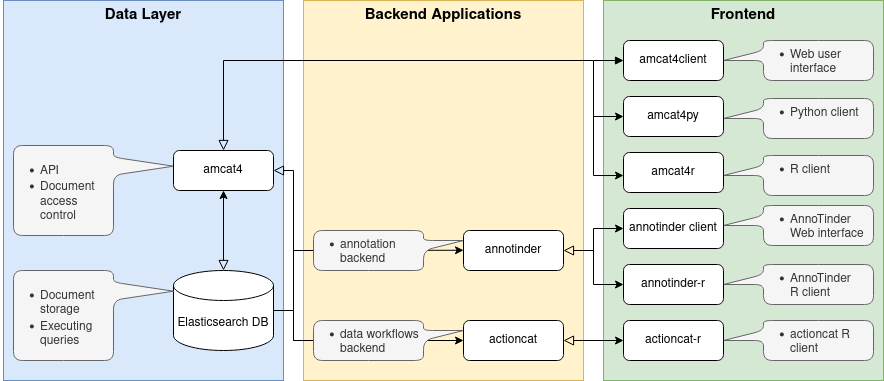
\includegraphics{media/amcat-flow.drawio.png}

}

\caption{The AmCAT4 design overview.\label{fig:design}}

\end{figure}

\hypertarget{web-interface-and-api}{%
\subsection{Web Interface and API}\label{web-interface-and-api}}

Instead of just showing how many documents are contained in a corpus,
AmCAT makes it possible to easily explore data before committing to it.
\autoref{fig:tax_parlee} shows the ParlEE data set (Sylvester, Greene,
and Ebing 2022), which consists of several gigabytes of csv files and
can be downloaded from the Harvard Dataverse. In AmCAT, it can be
explored by, for example, filtering for speeches in the Austrian
parliament that feature a term connected to migration. The example shows
that there is a stark increase in mentions of the terms in 2015, which
is probably interesting researchers focused on the migration debate.
Queries are made in \emph{Elasticsearch}'s ``mini-language'' for query
strings, which is widely used and
\href{https://web.archive.org/web/20230827002715/https://www.elastic.co/guide/en/elasticsearch/reference/current/query-dsl-query-string-query.html}{well
documented}.\footnote{\url{https://www.elastic.co/guide/en/elasticsearch/reference/current/query-dsl-query-string-query.html\#query-string-query-notes}}

\begin{figure}

{\centering \includegraphics{media/tax_parlee.png}

}

\caption{ParlEE data set on AmCAT web interface.\label{fig:tax_parlee}}

\end{figure}

Besides the web interface, we offer a fully featured REST API and API
wrapper packages for \texttt{R} and \texttt{Python}. We also include
OpenAPI specifications in the default installation, which makes it easy
to develop other wrappers. The API has the same search, upload,
download, and data modification capabilities as the web interface.
Below, we reproduce the search from \autoref{fig:tax_parlee} inside
\texttt{R}:

\begin{Shaded}
\begin{Highlighting}[]
\FunctionTok{library}\NormalTok{(tidyverse)}
\end{Highlighting}
\end{Shaded}

\begin{verbatim}
-- Attaching core tidyverse packages ------------------------ tidyverse 2.0.0 --
v dplyr     1.1.3     v readr     2.1.4
v forcats   1.0.0     v stringr   1.5.0
v ggplot2   3.4.2     v tibble    3.2.1
v lubridate 1.9.2     v tidyr     1.3.0
v purrr     1.0.2     
-- Conflicts ------------------------------------------ tidyverse_conflicts() --
x dplyr::filter() masks stats::filter()
x dplyr::lag()    masks stats::lag()
i Use the conflicted package (<http://conflicted.r-lib.org/>) to force all conflicts to become errors
\end{verbatim}

\begin{Shaded}
\begin{Highlighting}[]
\FunctionTok{library}\NormalTok{(amcat4r)}
\FunctionTok{amcat\_login}\NormalTok{(}\StringTok{"https://opted.amcat.nl/amcat"}\NormalTok{) }\CommentTok{\# publicly available server}
\FunctionTok{query\_documents}\NormalTok{(}
  \StringTok{"parlee"}\NormalTok{, }\CommentTok{\# name of the index}
  \AttributeTok{queries =} \StringTok{"(Google OR Amazon OR Starbucks OR Facebook OR twitter OR Apple) AND tax*"}\NormalTok{, }
  \CommentTok{\# include all fields}
  \AttributeTok{fields =} \ConstantTok{NULL}\NormalTok{,}
  \CommentTok{\# only search in Austrian corpus}
  \AttributeTok{filters   =} \FunctionTok{list}\NormalTok{(}\AttributeTok{iso3country =} \StringTok{"IRE"}\NormalTok{), }
  \AttributeTok{per\_page =} \DecValTok{10000}\NormalTok{, }
  \AttributeTok{page =} \ConstantTok{NULL}\NormalTok{, }\CommentTok{\# retrieve all pages}
  \AttributeTok{max\_pages =} \ConstantTok{Inf}
\NormalTok{) }\SpecialCharTok{|\textgreater{}} 
  \CommentTok{\# visualisation using ggplot2}
  \FunctionTok{count}\NormalTok{(date) }\SpecialCharTok{|\textgreater{}}
  \FunctionTok{ggplot}\NormalTok{(}\FunctionTok{aes}\NormalTok{(}\AttributeTok{x =}\NormalTok{ date, }\AttributeTok{y =}\NormalTok{ n)) }\SpecialCharTok{+}
  \FunctionTok{geom\_line}\NormalTok{()}
\end{Highlighting}
\end{Shaded}

\begin{verbatim}
\ Retrieved  results from page 0
v Retrieved 1539 results from page 1 [1.6s]
\end{verbatim}

\begin{figure}[H]

{\centering \includegraphics{paper_opted_files/figure-pdf/unnamed-chunk-1-1.pdf}

}

\end{figure}

The API makes AmCAT a valuable asset for power users and enables them to
include data in their reproduction materials. API commands can also be
used to in a script for larger-than-memory data, as chunks of the data
can be processed one by one instead of loading the whole data into
memory first.

\hypertarget{flexible-access-control}{%
\subsection{Flexible Access control}\label{flexible-access-control}}

An important feature of AmCAT is that it allows for fine-grained access
control and \emph{non-consumptive} research -- analyses that use
computational methods, while the researcher can not consume (i.e., read)
the text. This makes AmCAT the only easily available open source tool
(that we are aware of), which can enable researchers to share a corpus
in a way that users can query and visualize the data without being
granted access to the underlying text -- which circumvents most
copyright and ethical restrictions. We accomplish this with a set of
instance and index roles that allow the admin users to grant or revoke
access of indices (i.e., text collections), fields (columns) and the
AmCAT instance. What makes this special is that users can be granted
access to only to metadata of a text data set. For the queries an
searches a user can perform, this makes little difference. Only when
they try to read a text, they are presented with the message in
\autoref{fig:metareader}.

\begin{figure}

{\centering 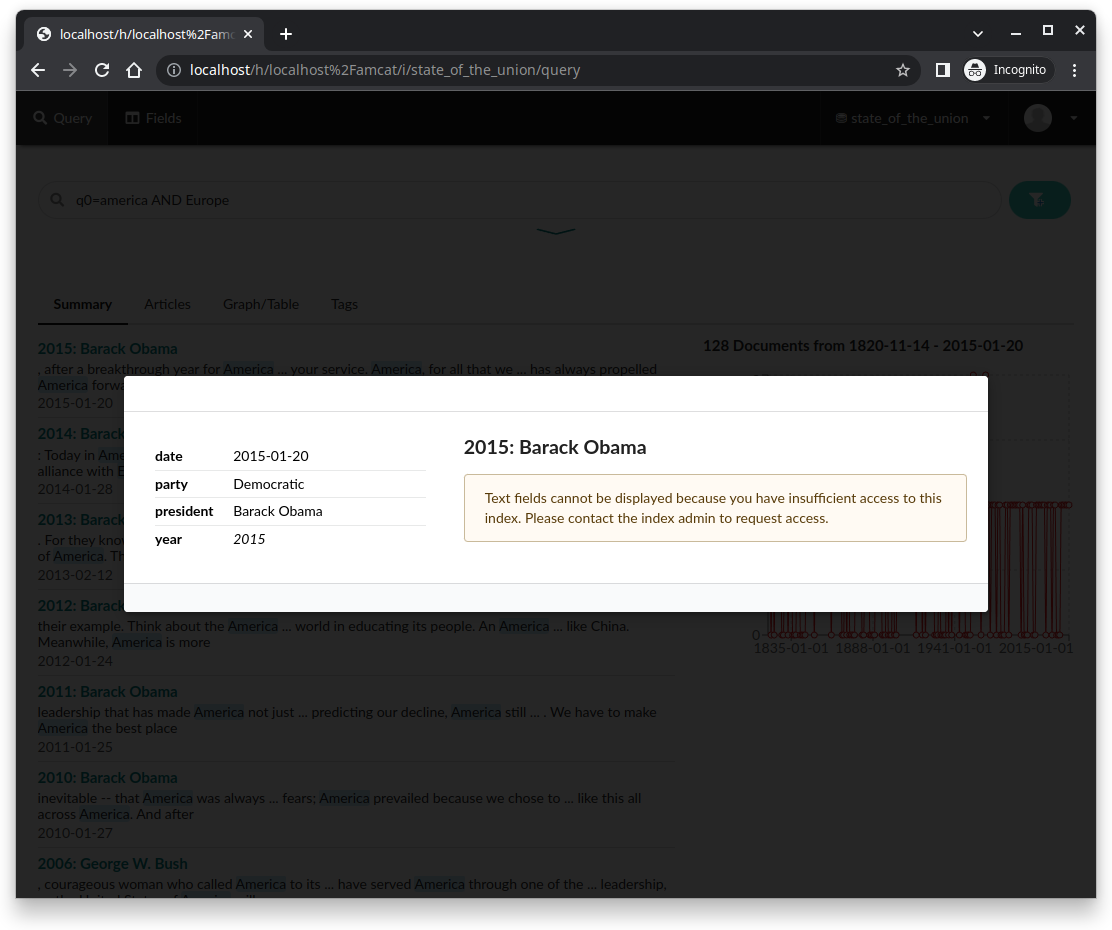
\includegraphics{media/sotu_text_guest.png}

}

\caption{`Metareader' users can query, but not read
text.\label{fig:metareader}}

\end{figure}

This setup allows for \emph{non-consumptive} research similar to the
functions of \emph{Google Books}, where researchers can check if a
corpus contains relevant data before working towards getting access. We
extend these capabilities by providing a framework to package arbitrary
workflows that can then be run on an AmCAT instance.

Using \texttt{actioncat}, users can write a script in \texttt{R},
\texttt{Python} or another language, package it into a Docker container
and send a Docker Compose file to the administrator of a server to check
if it conforms with theor policies on data access. Doing so enables
researchers to perform, for example, destructive pre-processing of text
(i.e., where the original text can not be restored). In this way, a
corpus can still be used for essentially every text-as-data analysis
pipeline imaginable, without running risk of violating copyrights or the
privacy of data owners. We provide two example workflows, one that uses
\texttt{R} to turn text into a document-feature-matrix, one that uses
\texttt{Python} to turn the text into document embeddings.

To authenticate users, we wrote our own authentication provider called
\texttt{middlecat}. Unlike in previous iterations, this completely omits
passwords in favor of connecting to identity providers like Github,
ORCID, or Google or one-time login links sent via e-mail. The advantage
is that we can follow a parsimonious approach to user privacy (besides
email addresses, we keep no user data) while still making sure that the
user is actually who they claim.

\hypertarget{installation-and-documentation}{%
\subsection{Installation and
Documentation}\label{installation-and-documentation}}

All different parts of AmCAT are publicly available on GitHub:

\begin{itemize}
\tightlist
\item
  \texttt{amcat4}: \url{https://github.com/ccs-amsterdam/amcat4}
\item
  \texttt{amcat4actioncat}:
  \url{https://github.com/ccs-amsterdam/amcat4actioncat}
\item
  \texttt{amcat4client}:
  \url{https://github.com/ccs-amsterdam/amcat4client}
\item
  \texttt{amcat4py}: \url{https://github.com/ccs-amsterdam/amcat4py}
\item
  \texttt{amcat4r}: \url{https://github.com/ccs-amsterdam/amcat4r}
\item
  \texttt{middlecat}: \url{https://github.com/ccs-amsterdam/middlecat}
\end{itemize}

The individual repositories contain instructions to install the
packages. We also provide a more comprehensive manual at
\url{https://amcat.nl/book/}, which covers installation, workflows, user
management and so on.

We recommend to install AmCAT through the open-source application
Docker. In our
\href{https://github.com/ccs-amsterdam/amcat4docker}{\texttt{amcat4docker}}
repository, we provide several Docker Compose files that make it
possible to get a full AmCAT instance running in minutes with no other
dependecies than Docker itself.

\hypertarget{refs}{}
\begin{CSLReferences}{1}{0}
\leavevmode\vadjust pre{\hypertarget{ref-ParlEE2022}{}}%
Sylvester, Christine, Zachary Greene, and Benedikt Ebing. 2022.
{``{ParlEE plenary speeches data set: Annotated full-text of 21.6
million sentence-level plenary speeches of eight EU states}.''} Harvard
Dataverse. \url{https://doi.org/10.7910/DVN/ZY3RV7}.

\end{CSLReferences}



\end{document}
